% figures-es/perceptual-map.tex
% Standalone TikZ: mapa perceptual 2x2 — precio vs facilidad de implementación,
%   categoría CRM de mercado medio (ch.04 segmentación-definición-posicionamiento).
% Compilado a figures-es/perceptual-map.pdf via tools/build-figures-es.sh.
\documentclass[tikz,border=6pt]{standalone}
\usepackage{tikz}
\usetikzlibrary{arrows.meta,positioning,calc}

\definecolor{vcblue}{HTML}{1A5276}
\definecolor{vcteal}{HTML}{0E6655}
\definecolor{vcgray}{HTML}{4D4D4D}
\definecolor{vcred}{HTML}{922B21}
\definecolor{vcamber}{HTML}{7D6608}

\begin{document}
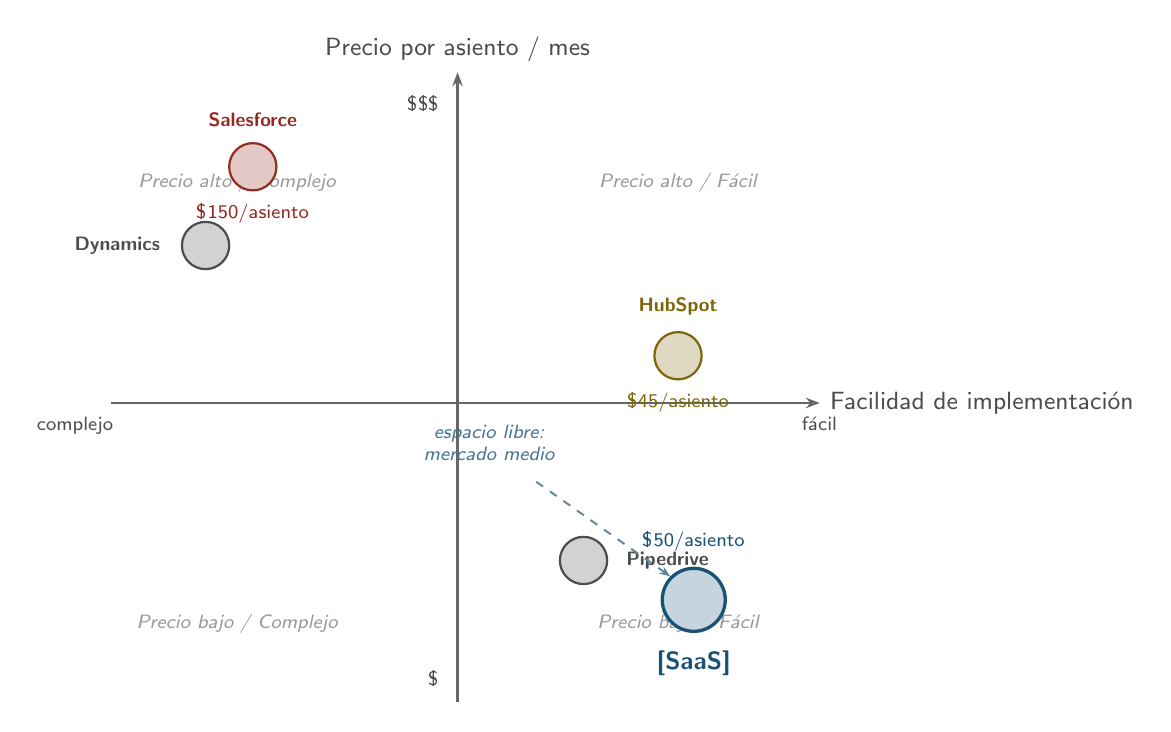
\begin{tikzpicture}[
  dot/.style={circle, draw=#1, fill=#1!25, line width=0.8pt,
              minimum size=6mm, font=\sffamily\scriptsize, text=black!85},
  axlbl/.style={font=\sffamily\small, text=black!70},
  quadlbl/.style={font=\sffamily\scriptsize\itshape, text=black!40},
]

%% ---- ejes ----
% eje x: Facilidad de implementación (izquierda=complejo, derecha=fácil)
% eje y: Precio por asiento/mes (abajo=bajo, arriba=alto)
\draw[-{Stealth[length=5pt]}, line width=0.9pt, black!60]
  (-4.4,0) -- (4.6,0) node[right, axlbl] {Facilidad de implementación};
\draw[-{Stealth[length=5pt]}, line width=0.9pt, black!60]
  (0,-3.8) -- (0,4.2) node[above, axlbl] {Precio por asiento / mes};

%% ---- etiquetas de marcas del eje ----
\node[axlbl, below left=2pt] at (-4.2,0) {\scriptsize complejo};
\node[axlbl, below right=2pt] at (4.2,0) {\scriptsize fácil};
\node[axlbl, left=3pt] at (0,-3.5) {\scriptsize \$};
\node[axlbl, left=3pt] at (0,3.8) {\scriptsize \$\$\$};

%% ---- etiquetas de cuadrantes ----
\node[quadlbl] at (-2.8, 2.8) {Precio alto / Complejo};
\node[quadlbl] at ( 2.8, 2.8) {Precio alto / Fácil};
\node[quadlbl] at (-2.8,-2.8) {Precio bajo / Complejo};
\node[quadlbl] at ( 2.8,-2.8) {Precio bajo / Fácil};

%% ---- puntos de competidores ----
% Salesforce: precio alto, implementación compleja
\node[dot=vcred] (sf) at (-2.6, 3.0)
  {\phantom{X}};
\node[font=\sffamily\scriptsize\bfseries, text=vcred, above=2pt of sf]
  {Salesforce};
\node[font=\sffamily\scriptsize, text=vcred, below=1pt of sf]
  {\$150/asiento};

% HubSpot: precio moderado, fácil — primero PYME
\node[dot=vcamber] (hs) at (2.8, 0.6)
  {\phantom{X}};
\node[font=\sffamily\scriptsize\bfseries, text=vcamber, above=2pt of hs]
  {HubSpot};
\node[font=\sffamily\scriptsize, text=vcamber, below=1pt of hs]
  {\$45/asiento};

% Microsoft Dynamics: precio alto, complejo
\node[dot=vcgray] (dyn) at (-3.2, 2.0)
  {\phantom{X}};
\node[font=\sffamily\scriptsize\bfseries, text=vcgray, left=4pt of dyn]
  {Dynamics};

% Pipedrive: precio bajo, facilidad moderada — PYME
\node[dot=vcgray] (pd) at (1.6, -2.0)
  {\phantom{X}};
\node[font=\sffamily\scriptsize\bfseries, text=vcgray, right=3pt of pd]
  {Pipedrive};

%% ---- punto de nuestra SaaS (destacado) ----
\node[dot=vcblue, minimum size=8mm, line width=1.2pt] (us) at (3.0, -2.5)
  {\phantom{X}};
\node[font=\sffamily\small\bfseries, text=vcblue, below=3pt of us]
  {[SaaS]};
\node[font=\sffamily\scriptsize, text=vcblue, above=2pt of us]
  {\$50/asiento};

%% ---- flecha de anotación de espacio en blanco ----
\draw[-{Stealth[length=4pt]}, vcblue!70, dashed, line width=0.7pt]
  (1.0,-1.0) -- (us.north west);
\node[font=\sffamily\scriptsize\itshape, text=vcblue!80, align=center]
  at (0.4,-0.5) {espacio libre:\\mercado medio};

\end{tikzpicture}
\end{document}
